\documentclass[]{beamer}
% hyperref={pdfpagelabels=false} in [] bei documentclass

\usepackage[utf8]{inputenc}
\usepackage[T1]{fontenc}
\usepackage[english]{babel}

\title{\Huge{$\mu-recursive~functions$}} % HASS HASS HASS VERKACKTES µ IM VERSCHISSENEN TITEL D:/
\author{Philip Geißler}
\date{17th of November}

\usetheme[progressbar=frametitle]{metropolis}
\usepackage{mathtools}

\begin{document}

\frame{\titlepage}

%\subsection{Introduction}
%f(x_1,x_2,\cdots,x_n) &= y \qquad\Longrightarrow& A(x_1,x_2,\cdots,x_n) &= y\\
%f(x_1,x_2,\cdots,x_n) &= y \qquad\Longrightarrow& A(x_1,x_2,\cdots,x_n) &= y

\addcontentsline{toc}{section}{Abstract: computability}
\begin{frame}{Abstract I}
	\begin{figure}[htb]
    	\includegraphics[height=6.5cm,width=10cm]{alice_bob.jpg}
		\caption{ ~Alice and Bob ~ \url{https://goo.gl/gRrDGH}}
	\end{figure}
\end{frame}

\begin{frame}{Abstract II}
\begin{center}
A function $f(x_1,x_2,\cdots,x_n)$ is computable if there exists an algoritm $A(x_1,x_2,\cdots,x_n)$ following given rules, that solves f in its domain and gives no output otherwise.\\
\begin{align*}
(x_1,x_2,\cdots,x_n) \in D_f &\Longrightarrow  A(x_1,x_2,\cdots,x_n) = f(x_1,x_2,\cdots,x_n)\\
(x_1,x_2,\cdots,x_n) \notin D_f &\Longrightarrow  A(x_1,x_2,\cdots,x_n) = \text{\textbf{ENDLESS LOOP}}
\end{align*}
\end{center}
\end{frame}

%\addcontentsline{toc}{section}{Table of Contents}
\begin{frame}{Table of contents}
%\setbeamertemplate{section in toc}[sections numbered]
\tableofcontents
\end{frame}

\begin{frame}{Abstract III}
well known computability models:
\begin{itemize}[<+->]
\item{turing machines}
\item{GOTO-programs}
\item{WHILE-programs}	\hspace{0.4cm}	$\supset$ LOOP-programs
\item{$\lambda$-calculus}
\item{\alert{$\mu$-recursive functions}} $\supset$ primitive recursive functions
\end{itemize}
\end{frame}

\section{$\mu$ - recursive functions}
\subsection{Definition and Disambiguation}

\begin{frame}{Definition}
\begin{center}
\textbf{Definition:}\\
The $\mu$-recursive
\only<2,8>{\begin{alert}}{functions}\only<2,8>{\end{alert}} are
\only<2,8>{\begin{alert}}{partial functions}\only<2,8>{\end{alert}} that return a
\only<3,8>{\begin{alert}}{single natural number}\only<3,8>{\end{alert}} and take
\only<3,8>{\begin{alert}}{finite tuples of natural numbers}\only<3,8>{\end{alert}}. They are the smallest class of
\only<2,8>{\begin{alert}}{partial functions}\only<2,8>{\end{alert}} that includes the
\only<4,8>{\begin{alert}}{initial functions}\only<4,8>{\end{alert}} and is closed under
\only<5,8>{\begin{alert}}{composition}\only<5,8>{\end{alert}},
\only<6,8>{\begin{alert}}{primitive recursion}\only<6,8>{\end{alert}}, and the
\only<7,8>{\begin{alert}}{$\mu$ operator}\only<7,8>{\end{alert}}.
\end{center}
\end{frame}

\begin{frame}{Disambiguation}
\begin{itemize}
\item{single and m-tupels of natural numbers}
\item{total and partial functions}
\item{initial functions}
	\begin{itemize}
	\item{constant function}
	\item{successor function}
	\item{projection function}
	\end{itemize}
\item{composition}
\item{primitive recursion}
\item{$\mu$ operator}
\end{itemize}
\end{frame}

\subsection{Basic mathematical understanding}

%\alert{\left\lbrace}0,1,2,3,\cdots\alert{\right\rbrace}
%\alert{\left(}n_1,n_2,n_3,\cdots,n_m\alert{\right)}

\begin{frame}{Single and m-tupels of natural numbers}
\begin{LARGE}
\only<1,2>{\begin{align*}
n &\in \mathbb{N} & \mathbb{N} &= \lbrace0,1,2,3,\cdots\rbrace
\end{align*}}
\only<1>{\begin{align*}
~\\
\end{align*}}
\only<2>{\begin{align*}
t &\in \mathbb{N}^m & t &= (n_1,n_2,n_3,\cdots,n_m)
\end{align*}}
\only<3>{
\begin{align*}
n &\in \mathbb{N} & \mathbb{N} &= \alert{\lbrace}0,1,2,3,\cdots\alert{\rbrace}
\end{align*}\\
\begin{align*}
t &\in \mathbb{N}^m & t &= \alert{(}n_1,n_2,n_3,\cdots,n_m\alert{ )}
\end{align*}}
\end{LARGE}
\only<1,2>{\center{\LARGE{~ ~\quad}}} % some chars that are seen as chars but do not show up
\only<3>{\center{\LARGE{tupels are not sets!}}}
\end{frame}

\begin{frame}{Total and partial functions}
\begin{align*}
L1&:=  \forall f_1,f_2 \in f: f(x)=f_1 \wedge f(x)=f_2 \Longrightarrow f_1=f_2\\
&\text{$\rightarrow$ each x has at most one corresponding f(x)}\\
\\
L2&:= \forall x \hspace{0.2cm} \exists f_1: f(x)=f_1 \\
&\text{$\rightarrow$ each x has at least one corresponding f(x)}
\end{align*}
\only<2>{\begin{align*}
f~&\hat=\text{ total function }&\Longrightarrow L1 = \text{true} &\wedge L2 = \text{true}\\
f~&\hat=\text{ partial function }&\Longrightarrow L1 = \text{true}&
\end{align*}}
\end{frame}

\subsection{Initial functions}

\begin{frame}{Constant function}
A function $N(x_1,x_2,\cdots,x_n)$ is a constant function if: \\
\begin{align*}
&& n,c &\in \mathbb{N} \\
N(x_1,x_2,\cdots,x_n) &= c & x_1,x_2,\cdots,x_n &\in \mathbb{N} \\
&&&
\end{align*}
\end{frame}

\begin{frame}{Successor function}
A function $S(x_1)$ is a successor function if: \\
\begin{align*}
&&& \\
S(x_1) &= x_1+1 & x_1 &\in \mathbb{N}  \\
&&&
\end{align*}
\end{frame}

\begin{frame}{Projection function}
A function $P_m^n(x_1,x_2,\cdots,x_n)$ is a projection function if: \\
\begin{align*}
&& n,m &\in \mathbb{N} \\
P_m^n(x_1,x_2,\cdots,x_m,\cdots,x_n) &= x_m & x_1,x_2,\cdots,x_n &\in \mathbb{N}  \\
&& 1\leqslant m&\leqslant n
\end{align*}
\end{frame}

\subsection{Composition function}

\begin{frame}{Composition function}
A function $C(x_1,x_2,\cdots,x_n)$ is a composition function if: \\
\begin{align*}
f_n &= f_n(x_1,x_2,\cdots,x_n) \\
f_{m,k} &= f_{m,k}(x_1,x_2,\cdots,x_m) \\
C &= f_n \circ (f_{m,1},f_{m,2},\cdots,f_{m,n})\\
&= f_n(f_{m,1}(x_{1,1},x_{1,2},\cdots,x_{1,m}),\cdots,f_{m,n}(x_{n,1},x_{n,2},\cdots,x_{n,m}))\\
\\
&n,m,x_{k,l } \in \mathbb{N}
\end{align*}
\end{frame}

\subsection{Primitive recursion function}

\begin{frame}{Primitive recursion function}
A function $R(X_0,x_1,x_2,\cdots,x_n)$ is primitive recursive if: \\
\begin{align*}
X_0=0 \Longrightarrow ~ R(X_0,x_1,x_2,\cdots,x_n) &= f(y_1,\cdots,y_m)\\
X_0\neq0 \Longrightarrow ~ R(X_0,x_1,x_2,\cdots,x_n) &= g(R(X_0-1,x_1,\cdots,x_n),z_1,\cdots,z_l)\\
\\
x_k,y_k,z_k,n,m,l &\in \mathbb{N}
\end{align*}
\end{frame}

\begin{frame}{Digression: primitive recursive functions}
Example:
\begin{align*}
f(x,y,z) &= (x\cdot y)^2-z & x,y,z &\in \mathbb{N}\\
\end{align*}
\end{frame}

\begin{frame}{Digression: primitive recursive functions}
\begin{align*}
f(x,y,z) &= (x\cdot y)^2-z & x,y,z &\in \mathbb{N}\\
\end{align*}
Basic functions we need for f(x,y,z):
\only<1>{\begin{align*}
add(x,y) &= x+y~,~ mult(x,y) = x*y\\
add(x,y) &=
\begin{cases}
add(0,y) &= y\\
add(x+1,y) &= S(add(x,y))
\end{cases}\\
mult(x,y) &=
\begin{cases}
mult(0,y) &= 0\\
mult(x+1,y) &= add(mult(x,y),y)
\end{cases}
\end{align*}}
\only<2>{\begin{align*}
decr(x,y) &= x-1~,~ sub(x,y) = x-y\\
decr(x) &=
\begin{cases}
decr(0) &= 0\\
decr(x+1) &= x
\end{cases}\\
sub(x,y) &=
\begin{cases}
sub(x,0) &= x\\
sub(x,y+1) &= decr(sub(x,y))
\end{cases}
\end{align*}}
\end{frame}

\begin{frame}{Digression: primitive recursive functions}
\begin{align*}
mult(x,y) &= x*y & sub(x,y) &= x+y & mult,sub \in Primitive~RF
\end{align*}
\begin{align*}
f(x,y,z) &= (x\cdot y)^2-z & x,y,z &\in \mathbb{N}\\
\only<2,3,4,5,6>{&= mult(x,y)^2-z}~\\
\only<3,4,5,6>{&= mult(x,y) \cdot mult(x,y) - z}~\\
\only<4,5,6>{&= mult(mult(x,y),mult(x,y)) -z}~\\
\only<5,6>{&= sub(mult(mult(x,y),mult(x,y)),z)}~\\\\
\only<6>{&= sub(mult(mult(P_1^3(x,y,z),P_2^3(x,y,z)),\\
& ~~~~mult(P_1^3(x,y,z),P_2^3(x,y,z))),P_3^3(x,y,z))}~\\
\end{align*}
\end{frame}

\subsection{$\mu$ minimisation function}

\begin{frame}{$\mu$ minimisation function}
A function $\mu(f(Y_0,y_1,y_2,\cdots,y_n),x_1,x_2,\cdots,x_n)$ is $\mu$ minimizing if: \\
\begin{align*}
0 &= f(z,y_1,y_2,\cdots,y_n) \\
\wedge~ 0 &< f(i,y_1,y_2,\cdots,y_n) &0\leqslant i< z\\
\Longleftrightarrow n &= \mu(f(Y_0,y_1,y_2,\cdots,y_n),x_1,x_2,\cdots,x_n) \\
\\
&n,z,i_k,y_k \in \mathbb{N}
\end{align*}
\end{frame}

\begin{frame}{Pseudoxample $\mu$ recursive function}
Example:
\begin{align*}
Z_f &= undef,undef,undef,0,1,2,3,\cdots\\
\\
\Longrightarrow f(x) &=
\begin{cases}
undef &| x\leqslant 2\\
x-3 &| x \geqslant 3
\end{cases}
\end{align*}
\end{frame}

\begin{frame}{Pseudoxample $\mu$ recursive function}
\begin{align*}
f(x) &=
\begin{cases}
undef &| x\leqslant 2\\
n-3 &| x \geqslant 3
\end{cases}
\end{align*}
Basic functions we need for f(x,y,z):
\only<1>{
\begin{align*}
decr(x) &=
\begin{cases}
decr(0) &= 0\\
decr(x+1) &= x
\end{cases}\\
sub(x,y) &=
\begin{cases}
sub(x,0) &= x\\
sub(x,y+1) &= decr(sub(x,y))
\end{cases}
\end{align*}}
\only<2>{
\begin{align*}
3sub(z,x) &= sub(sub(z,3),x)\\
&= z-3-x\\
\Longrightarrow\mu(3sub(z,x)) &= \text{smallest natural x with given z,}\\
&\qquad \text{for that }3sub(z,x)=0 \Rightarrow\\
z=0 &\leftrightarrow undef,
z=1 \leftrightarrow undef,\\
z=2 &\leftrightarrow undef,
z=3 \leftrightarrow 0, z=4 \leftrightarrow 1, \cdots \\
\Longrightarrow f(x)
\end{align*}}
\end{frame}

\section{Appendix: computability}

\begin{frame}{Abstract IV}
\only<3>{class relations between the different complete computability models:}
\begin{figure}[h]
\begin{tikzpicture}[scale=1.3]
\node (A) at (-2,1){$\mu$ - recursive functions};
\node (B) at (2,1){primitive recursive functions};
\only<2,3>{\node (C) at (2,0){LOOP-programs};}
\only<2,3>{\node (D) at (-2,0){WHILE-programs};}
\only<3>{\node (E) at (-4,-1){GOTO-programs};}
\only<3>{\node (F) at (-1,-1){Turing machines};}

\draw[<-] (A) edge (B);
\only<2,3>{\draw[<->] (A) edge (D);}
\only<2,3>{\draw[<->] (C) edge (B);}
\only<2,3>{\draw[->] (C) edge (D);}
\only<3>{\draw[<->] (D) edge[bend right=30] (E);}
\only<3>{\draw[<->] (F) edge[bend right=30] (D);}
\only<3>{\draw[<->] (E) edge[bend right=30] (F);}

\end{tikzpicture}
\end{figure}
\end{frame}

\begin{frame}{Abstract V}
\only<2>{class relations between the different complete computability models:\\
~\\}
\begin{figure}[h]
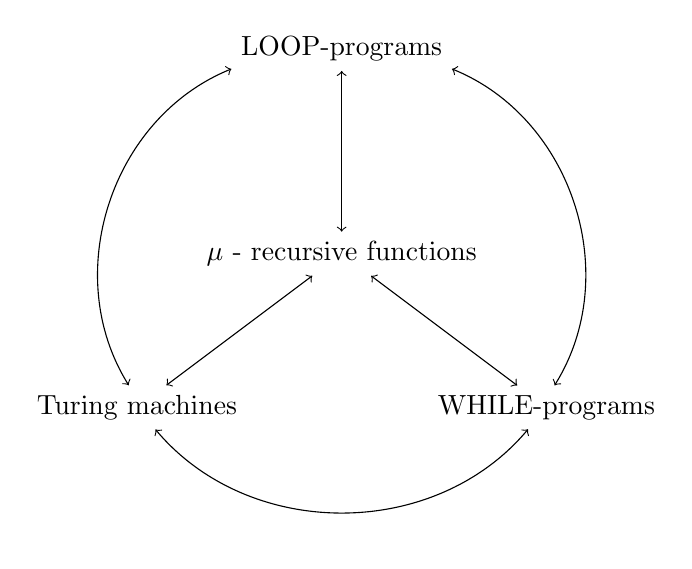
\begin{tikzpicture}[scale=1.3]
\node (A) at (0,0){$\mu$ - recursive functions};
\only<2>{\node (x) at (0,2){LOOP-programs};}
\only<2>{\node (y) at (2,-1.5){WHILE-programs};}
\only<2>{\node (z) at (-2,-1.5){Turing machines};}

\only<2>{\draw[<->] (A) edge (x);}
\only<2>{\draw[<->] (A) edge (y);}
\only<2>{\draw[<->] (A) edge (z);}

\only<2>{\draw[<->] (x) edge[bend left=50] (y);}
\only<2>{\draw[<->] (y) edge[bend left=50] (z);}
\only<2>{\draw[<->] (z) edge[bend left=50] (x);}

\end{tikzpicture}
\end{figure}
\end{frame}

\begin{frame}{Sources}
Access Date:
			\today
\begin{thebibliography}{xxxx}

		\bibitem[Picture]{}
		The picture in the introduction\\
			URL: \url{https://goo.gl/gRrDGH}
		\bibitem[Overall]{}
		Explanations of subtopics of µ-recursion\\
			URL: \url{https://goo.gl/yWvinS}\\
			URL: \url{https://goo.gl/xRPCiU}\\
			URL: \url{https://goo.gl/K4LKQB}\\
			URL: \url{https://goo.gl/XudPdL}
		\bibitem[Overall]{}
			U.Schöning, Theoretische Informatik kurz gefasst, 2008, Spektrum

\end{thebibliography}
\end{frame}

\begin{frame}
\maketitle
\end{frame}

\end{document}
